\documentclass[14pt,a4paper,report]{report}
\usepackage[a4paper, mag=1000, left=2.5cm, right=1cm, top=2cm, bottom=2cm, headsep=0.7cm, footskip=1cm]{geometry}
\usepackage[utf8]{inputenc}
\usepackage[english,russian]{babel}
\usepackage{indentfirst}
\usepackage[dvipsnames]{xcolor}
\usepackage[colorlinks]{hyperref}
\usepackage{listings} 
\usepackage{fancyhdr}
\usepackage{caption}
\usepackage{graphicx}
\hypersetup{
	colorlinks = true,
	linkcolor  = black
}

\usepackage{titlesec}
\titleformat{\chapter}
{\Large\bfseries} % format
{}                % label
{0pt}             % sep
{\huge}           % before-code


\DeclareCaptionFont{white}{\color{white}} 

% Listing description
\usepackage{listings} 
\DeclareCaptionFormat{listing}{\colorbox{gray}{\parbox{\textwidth}{#1#2#3}}}
\captionsetup[lstlisting]{format=listing,labelfont=white,textfont=white}
\lstset{ 
	% Listing settings
	inputencoding = utf8,			
	extendedchars = \true, 
	keepspaces = true, 			  	 % Поддержка кириллицы и пробелов в комментариях
	language = bash,            	 	 % Язык программирования (для подсветки)
	basicstyle = \small\sffamily, 	 % Размер и начертание шрифта для подсветки кода
	numbers = left,               	 % Где поставить нумерацию строк (слева\справа)
	numberstyle = \tiny,          	 % Размер шрифта для номеров строк
	stepnumber = 1,               	 % Размер шага между двумя номерами строк
	numbersep = 5pt,              	 % Как далеко отстоят номера строк от подсвечиваемого кода
	backgroundcolor = \color{white}, % Цвет фона подсветки - используем \usepackage{color}
	showspaces = false,           	 % Показывать или нет пробелы специальными отступами
	showstringspaces = false,    	 % Показывать или нет пробелы в строках
	showtabs = false,           	 % Показывать или нет табуляцию в строках
	frame = single,              	 % Рисовать рамку вокруг кода
	tabsize = 2,                  	 % Размер табуляции по умолчанию равен 2 пробелам
	captionpos = t,             	 % Позиция заголовка вверху [t] или внизу [b] 
	breaklines = true,           	 % Автоматически переносить строки (да\нет)
	breakatwhitespace = false,   	 % Переносить строки только если есть пробел
	escapeinside = {\%*}{*)}      	 % Если нужно добавить комментарии в коде
}

\begin{document}

\def\contentsname{Contents}

% Titlepage
\begin{titlepage}
	\begin{center}
		\textsc{Peter the Great St.Petersburg Polytechnic University\\[5mm]
			Department of Computer Systems \& Software Engineering}
		
		\vfill
		
		\textbf{Laboratory report №2\\[3mm]
			Discipline: «Information Security»\\[3mm]
			Theme: «Network Mapper»\\[41mm]
		}
	\end{center}
	
	\hfill
	\begin{minipage}{.4\textwidth}
		Made by student:\\[2mm] 
		Boyarkin N.S.\\
		Group: 13541/3\\[5mm]
		
		Lecturer:\\[2mm] 
		Bogach N.V.
	\end{minipage}
	\vfill
	\begin{center}
		Saint-Petersburg\\ \the\year\ y.
	\end{center}
\end{titlepage}

% Contents
\tableofcontents
\clearpage

\chapter{Laboratory work №2}

\section{Work purpose}

Study nmap utility with help of Kali Linux and Metasploitable2 VM.

\section{Task}

\begin{enumerate}
	\item List targets to scan.
	\item Probe open ports to determine service/version info.
	\item Study nmap-services, nmap-os-db, nmap-service-probes.
	\item Add new service to nmap-service-probes (create a minimal tcp server, get its name and version by nmap).
	\item Study nmap stages and modes using Wireshark.
	\item Output to xml-format file.
	\item Perform VM Metasploitable2 scanning using db\_nmap from metasploitframework.
	\item Get some records from nmap-service-probes and describe them. Choose one Nmap Script and describe it.
\end{enumerate}

\clearpage

\section{Work Progress}

\subsection{Introduction}

Nmap uses raw IP packets in novel ways to determine what hosts are availableon the network, what services (application name and version) those hosts are offering, what operating systems (and OS versions) they are running, what type of packet filters/firewalls are in use, and dozens of other characteristics. It was designed to rapidly scan large networks, but works fine against single hosts. Nmap runs on all major computer operating systems, and official binary packages are available for Linux, Windows, and Mac OS X.

\subsection{Creating connection}

We used three operating systems at this laboratory work:

\begin{enumerate}
	\item \textbf{Kali Linux} -- VM, IP: 192.168.56.102
	\item \textbf{Metasploitable 2} -- VM, IP: 192.168.56.101
	\item \textbf{Windows 10} -- Real, IP: 192.168.56.1
\end{enumerate}

The following code obtains the network configuration for Kali Linux:

\lstinputlisting{listings/1.log}

Network configuration for Metasploitable 2:

\begin{figure}[h!]
	\centering
	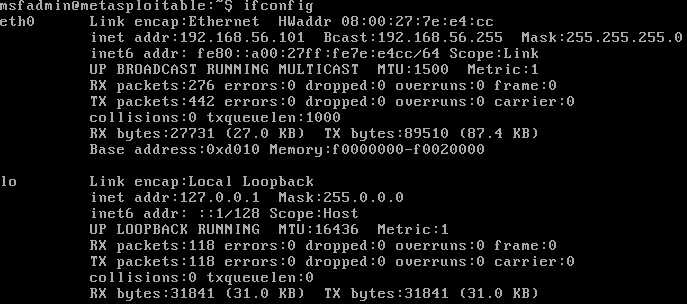
\includegraphics[scale = 0.90]{images/1.png}
	\caption{Metasploitable 2 network configuration}
\end{figure}

\clearpage

Let's try to check connection between Kali and Metasploitable 2 by the browser:

\begin{figure}[h!]
	\centering
	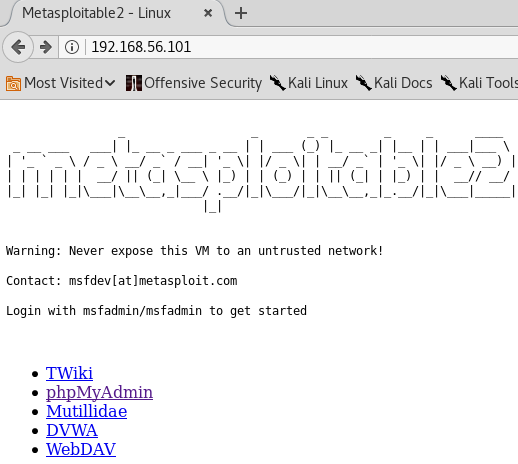
\includegraphics[scale = 0.60]{images/2.png}
	\caption{Connection from Kali to Metasploitable 2 established}
\end{figure}

Ping also going well:

\begin{figure}[h!]
	\centering
	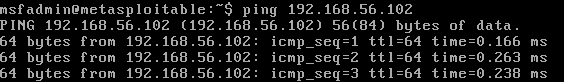
\includegraphics[scale = 0.68]{images/3.png}
	\caption{Connection from Metasploitable 2 to Kali established}
\end{figure}

\subsection{List targets to scan}

Let's start scaning Metasploitable 2 OS by the \textbf{nmap} utility. Option \textbf{-n} initiates fast scan (without port scanning). The main argument of the nmap utility is IP address (or range) of the remote host.

\lstinputlisting{listings/3.1.log}

\subsection{Probe open ports to determine service/version info}

Option \textbf{-top-ports} searches for the most used ports of the remote machine. Let's compare the result of nmap utility for the Metasploitable 2 OS and Windows 10 OS.

\lstinputlisting{listings/3.2.log}

Metasploitable 2 has many vulnerabilities, including open ports without filtering. At the same time Windows has a built-in firewall, that filters some nmap packets.

Option \textbf{-V} used to display versions of the protocols:

\lstinputlisting{listings/4.log}

This experiment shows that remote attackers can get a lot of information about the system, so to ensure security, you must use a firewall.

\subsection{Study nmap-services, nmap-os-db, nmap-service-probes}

The utility files for nmap can be found in the directory \textbf{/usr/share/nmap}.

The \textbf{nmap-services} file is a registry of port names to their corresponding number and protocol. Each entry has a number representing how likely that port is to be found open. Most lines have a comment as well. Nmap ignores the comments, but users sometimes grep for them in the file when Nmap reports an open service of a type that the user does not recognize.

\lstinputlisting{listings/5.log}

The \textbf{nmap-os-db data} file contains hundreds of examples of how different operating systems respond to Nmap's specialized OS detection probes. It is divided into blocks known as fingerprints, with each fingerprint containing an operating system's name, its general classification, and response data.

\lstinputlisting{listings/6.log}

While the version of nmap-services distributed with Nmap is sufficient for most users, understanding the file format allows advanced Nmap hackers to add their own services to the detection engine. Like many Unix files, \textbf{nmap-service-probes} is line-oriented. Lines starting with a hash (\#) are treated as comments and ignored by the parser. Blank lines are ignored as well. Other lines must contain one of the directives described below.

\lstinputlisting{listings/7.log}

\subsection{Add new service to nmap-service-probes}

Let's start simple TCP echo server by the following C++ code:

\lstinputlisting{listings/8.cpp}

Compile and run the server on port 65100:

\lstinputlisting{listings/9.log}

Let's try to check \textbf{nmap} result before changes into nmap-service-probes file:

\lstinputlisting{listings/10.log}

The results indicate that it was not possible to determine the type of port and application.

The echo server displays information about requests coming to it. This illustrates the operating principle of the \textbf{nmap} utility: various requests are sent and depending on the response, the type of protocol is determined.

\lstinputlisting{listings/12.log}

The following code was added to the \textbf{nmap-service-probes} file, which will help \textbf{nmap} determine the type and version of the application:

\lstinputlisting{listings/11.log}

After this changes \textbf{nmap} successfully recognize the type of protocol:

\lstinputlisting{listings/13.log}

\subsection{Study nmap stages and modes using Wireshark}

Consider the network interaction of the utility nmap in the Wireshark program. Let's try to get 5 most used ports of Metasploitable 2 OS:

\begin{verbatim}
root@kali:~# nmap -sV -top-ports 5 192.168.56.101
\end{verbatim}

\begin{figure}[h!]
	\centering
	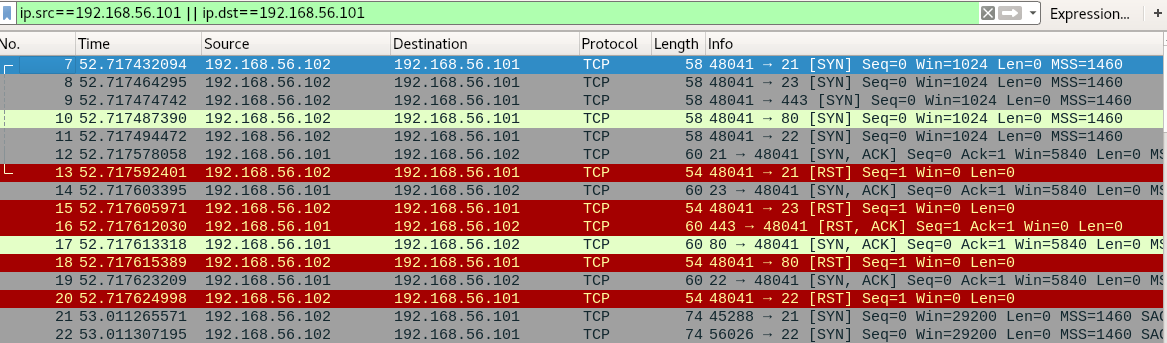
\includegraphics[scale = 0.53]{images/4.png}
	\caption{Trying to get 5 most used ports}
\end{figure}

Nmap tries to establish TCP connections with a lot of ports on the target system. if a packet with the RST flag is returned, the namp concludes that the port is closed. If no response is received, then the port is filtered or does not exist.

Let's try to get information about the TCP server, that is running on port 65100:

\begin{verbatim}
msfadmin@metasploitable:~$ nmap -sV -p 65100 192.168.56.102
\end{verbatim}

\begin{figure}[h!]
	\centering
	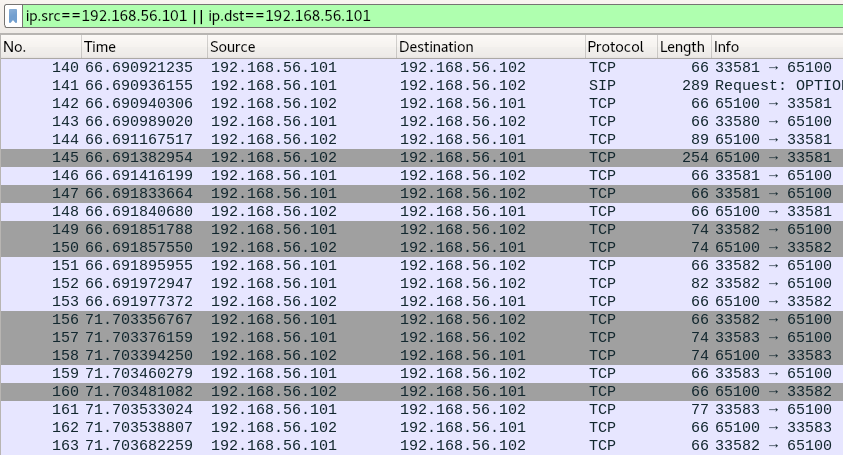
\includegraphics[scale = 0.53]{images/5.png}
	\caption{Trying to get information about port 65100}
\end{figure}

This illustrates the operating principle of the \textbf{nmap} utility: various requests are sent and depending on the response, the type of protocol is determined.

\subsection{Output to xml-format file}

The result of the operation can be represented in the XML format:

\lstinputlisting{listings/14.log}

\subsection{Perform VM Metasploitable2 scanning using db\_nmap from metasploitframework}

We can use the db\_nmap command to run Nmap against our targets and our scan results would than be stored automatically in our database. However, if you also wish to import the scan results into another application or framework later on, you will likely want to export the scan results in XML format.

\lstinputlisting{listings/15.log}

\subsection{Get some records from nmap-service-probes and describe them}

\begin{verbatim}
Probe <protocol> <probename> <probestring>
\end{verbatim}

The Probe directive tells Nmap what string to send to recognize various services. All of the directives discussed later operate on the most recent Probe statement. The arguments are as follows:

\begin{itemize}
	\item \textbf{<protocol>} -- This must be either TCP or UDP. Nmap only uses probes that match the protocol of the service it is trying to scan.
	\item \textbf{<probename>} -- This is a plain English name for the probe. It is used in service fingerprints to describe which probes elicited responses.
	\item \textbf{<probestring>} -- Tells Nmap what to send.
\end{itemize}


\begin{verbatim}
match <service> <pattern> [<versioninfo>]
\end{verbatim}

The match directive tells Nmap how to recognize services based on responses to the string sent by the previous Probe directive. The arguments to this directive follow:

\begin{itemize}
	\item \textbf{<service>} -- This is simply the service name that the pattern matches.
	\item \textbf{<pattern>} -- This pattern is used to determine whether the response received matches the service given in the previous parameter.
	\item \textbf{<versioninfo>} -- actually contains several optional fields. Each field begins with an identifying letter (such as h for "hostname"). Next comes a delimiter character which the signature writer chooses.
\end{itemize}

\begin{verbatim}
rarity <value between 1 and 9>
\end{verbatim}

The rarity directive roughly corresponds to how infrequently this probe can be expected to return useful results. The higher the number, the more rare the probe is considered and the less likely it is to be tried against a service.

\begin{verbatim}
ports <portlist>
\end{verbatim}

This line tells Nmap what ports the services identified by this probe are commonly found on. It should only be used once within each Probe section.

\subsection{Choose one Nmap Script and describe it}

The Nmap Scripting Engine (NSE) is one of Nmap's most powerful and flexible features. It allows users to write (and share) simple scripts to automate a wide variety of networking tasks. Those scripts are then executed in parallel with the speed and efficiency you expect from Nmap. Users can rely on the growing and diverse set of scripts distributed with Nmap, or write their own to meet custom needs.

The following script starts all unit tests for the nmap utility and located at /usr/share/nmap/scripts/unittest.nse:

\lstinputlisting{listings/16.nse}

This script contains the following fields:

\begin{itemize}
	\item \textbf{description} -- describes what a script is testing for and any important notes the user should be aware of.
	\item \textbf{author} -- contains the script authors' names and can also contain contact information.
	\item \textbf{license} -- helps ensure that we have legal permission to distribute all the scripts which come with Nmap.
	\item \textbf{categories} -- defines one or more categories to which a script belongs.
	\item \textbf{prerule} -- determines whether a script should be run against a target. Prerule run once, before any hosts are scanned, during the script pre-scanning phase.
	\item \textbf{action} -- contains all of the instructions to be executed when the script's prerule, portrule, hostrule or postrule triggers.
\end{itemize}

\section{Conclusion}

Nmap is a free and open source utility for network discovery and security auditing. In this laboratory work, the main features of this utility were studied, and experiments were performed to illustrate its power. All these experiments show that remote attackers can get a lot of information about the system, so to ensure security, you must use a firewall.

\end{document}